\documentclass[a4paper, 12pt, margin= 1.25cm ]{article}

\title{Scientific Python}
\date{02-02-2018}
\author{Milind Kumar V\\ EE16B025}

\usepackage{color}
\usepackage{graphicx}
\usepackage{listings}
\usepackage{amsmath}
\usepackage{float}
\usepackage{longtable}
\usepackage[utf8]{inputenc}
\usepackage[T1]{fontenc}
\usepackage{booktabs}

\definecolor{back}{rgb}{0.96,0.96,0.96}

\lstset{ %
  backgroundcolor=\color{back},   % choose the background color; you must add \usepackage{color} or \usepackage{xcolor}; should come as last argument
  basicstyle=\footnotesize,        % the size of the fonts that are used for the code
  breakatwhitespace=false,         % sets if automatic breaks should only happen at whitespace
  breaklines=true,                 % sets automatic line breaking
  captionpos=b,                    % sets the caption-position to bottom
  commentstyle=\color{black},    % comment style
  deletekeywords={...},            % if you want to delete keywords from the given language
  escapeinside={\%*}{*)},          % if you want to add LaTeX within your code
  extendedchars=true,              % lets you use non-ASCII characters; for 8-bits encodings only, does not work with UTF-8
  frame= single,	                   % adds a frame around the code
  keepspaces=true,                 % keeps spaces in text, useful for keeping indentation of code (possibly needs columns=flexible)
  keywordstyle=\color{black},       % keyword style
  language=Python,                 % the language of the code
  morekeywords={*,...},            % if you want to add more keywords to the set
  numbers=left,                    % where to put the line-numbers; possible values are (none, left, right)
  numbersep=5pt,                   % how far the line-numbers are from the code
  numberstyle=\tiny\color{black}, % the style that is used for the line-numbers
  rulecolor=\color{black},         % if not set, the frame-color may be changed on line-breaks within not-black text (e.g. comments (green here))
  showspaces=false,                % show spaces everywhere adding particular underscores; it overrides 'showstringspaces'
  showstringspaces=false,          % underline spaces within strings only
  showtabs=false,                  % show tabs within strings adding particular underscores
  stepnumber=1,                    % the step between two line-numbers. If it's 1, each line will be numbered
  stringstyle=\color{black},     % string literal style
  tabsize=2,	                   % sets default tabsize to 2 spaces
  title=\lstname                   % show the filename of files included with \lstinputlisting; also try caption instead of title
}



\begin{document}
	\pagenumbering{gobble}
	\maketitle
	\newpage
	\pagenumbering{arabic}
	
	\begin{abstract}
	This report presents an elementary study of the two primary modules used in scientific python, namely Scipy and Numpy. The various ways to determine running integrals using the definition of $tan^{-1}x$ as a definite integral are explored. This is further done using the Trapezoidal Rule setting a tolerance of $10^{-8}$ and subsequent error estimates are plotted.
	\end{abstract}
	\section{Introduction}     
	This report presents three ways of obtaining the values of the function $tan^{-1}x$ at various values of $x$ one of which is using the $quad$ function in the scipy module. The following relation is used to obtain the value of $tan^{-1}x$ over at any x
		\begin{equation*}\label{equation1}
		tan^{-1}x= \int^x_0 \frac{du}{1+u^2}
		\end{equation*}
	The error in the values of $tan^{-1}x$ is measured by comparing the values returned by the $arctan$ function $arctan$ in numpy and is plotted. Subsequently, a strategy using the trapezoid rule is devised to compute the aforementioned integral. A comparision of the results of vectorisation of the code and the use of a for loop is also made.

	\section{Methods and results}
	The functions necessary for this exercise have been wriiten in a separate file and thus necessicate making making the following imports.

		\begin{lstlisting}

		from __future__ import division
		import numpy as np
		from matplotlib import pyplot as plt
		from functions import function1, taninv, trapezoid_integrate, trapezoid_integrate_for_loop
		
		\end{lstlisting}

	This first section deals with the necessary imports with the $functions$ referring to the document in which the functions necessary for this assignement are stored. The following are the imports in the functions file.

		\begin{lstlisting}
		
		from __future__ import division

		import numpy as np
		from scipy.integrate import quad
		\end{lstlisting}	

	The second line of code above helps remove the ambiguity around the $/$ operator in Python.

	\begin{enumerate}
		\item A function is made to compute the values $1/(1+u^2)$ and given a vector, to return this value for every element of the vector.
		
		\begin{lstlisting}
		
		def function1(a):
		a= np.array(a)
		return 1.0/(1.0+a**2)

		\end{lstlisting}

		\item A vector of values is made for the above function to be tested upon using the following code.

		\begin{lstlisting}
		
		# Step 2


		start= 0.0
		stop= 5.0
		num= 51									
		# to include the last element and avoid obo error
		vector= np.linspace(start, stop, num)	# calling x vector


		values= function1(vector)
				
		\end{lstlisting}		

		\item This vector is passed to the above function and the returned values for $1/(1+u^2)$ are subsequently plotted using the matplotlib module.

		\begin{lstlisting}
		
		
		##########
		# Step 3

		plt.plot(vector, values, "bo")
		plt.xlabel("x")
		plt.ylabel("$f(x)$")
		plt.title("""Plot of $f(x) = 1/(1+x^2) $""")
		plt.show()
		plt.close()

				
		\end{lstlisting}		

		
		\begin{figure}[h!]
			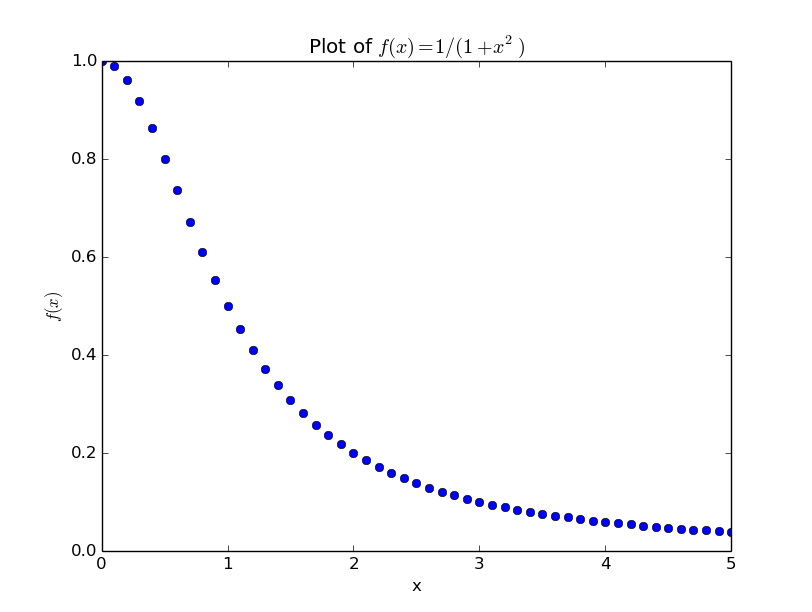
\includegraphics[width= \linewidth]{figure0.png}
			\label{fig:figure0}
			\caption{A plot of $f(x)$ vs $x$}
		\end{figure}
		
		Figure \ref{fig:figure0} shows the plot of $f(x)= 1/(1+x^2)$ which decays with x as is expected. We now define $I(x)= tan^{-1}x$ as follows
			\begin{equation}\label{eq:i}
			I(x)= tan^{-1}x= \int^x_0f(x)dx= \int^x_0 dx/(1+x^2)
			\end{equation}		

		\item The values of $I(x)$ are computed for vector which we have defined beforehand using the $quad$ function from scipy.integrate. This function returns a tuple which is subsequently converted to a numpy array and returned to the calling function $taninv$. We consider the first column vector for the returned values of $tan^{-1}x$. The following code describes the $taninv$ function from functions.py.
		
		\begin{lstlisting}

		def taninv(a):
		a= np.array(a)
		array= []
		for i in a:
			array.append(quad(function1, 0.0, i))
		array= np.array(array)
	#	array[:,0] = [round(i,5) for i in array[:,0]]	
		return (array)		
		
		\end{lstlisting}		

		The following code computes the error and makes a plot of $I(x)$ and the $np.arctan$ function from the numpy library and the error between the two.

		\begin{lstlisting}

		###########
		# Step 4

		taninv_calculated= np.array(taninv(vector)[:,0])	
		# remember that the quad function 
		# returns (integral, error)
		taninv_actual= np.arctan(vector)
		error= taninv_calculated- taninv_actual




		plt.figure(1)

		plt.subplot(211)
		plt.plot( vector, taninv_calculated, "ro", label= "quad")
		plt.plot( vector, taninv_actual, "k-", label="$tan^{-1}(x)$", linewidth=2)
		plt.xlabel("x")
		plt.ylabel("$\int^x_0 du/(1+u^2) $")
		plt.title("A comparision of quad and np.arctan()")
		plt.legend(loc= "lower right")

		plt.subplot(212)
		plt.semilogy(vector, error, "ro")
		plt.xlabel("x")
		plt.ylabel("Error")
		plt.title("Error in $\int^x_0 dx/(1+x^2) $")
		plt.tight_layout()
		plt.show()
		plt.close()



		plt.semilogy(vector, (taninv(vector))[:,1], "ro")
		plt.xlabel("x")
		plt.ylabel("Error from quad")
		plt.title("Error returned by the quad function")

		plt.tight_layout()	# ensures reasonable gaps between 
							# the first subplot and the second				
		plt.show()

		plt.close()

		\end{lstlisting}

		This results in the following plot.

		\begin{figure}[h!]
		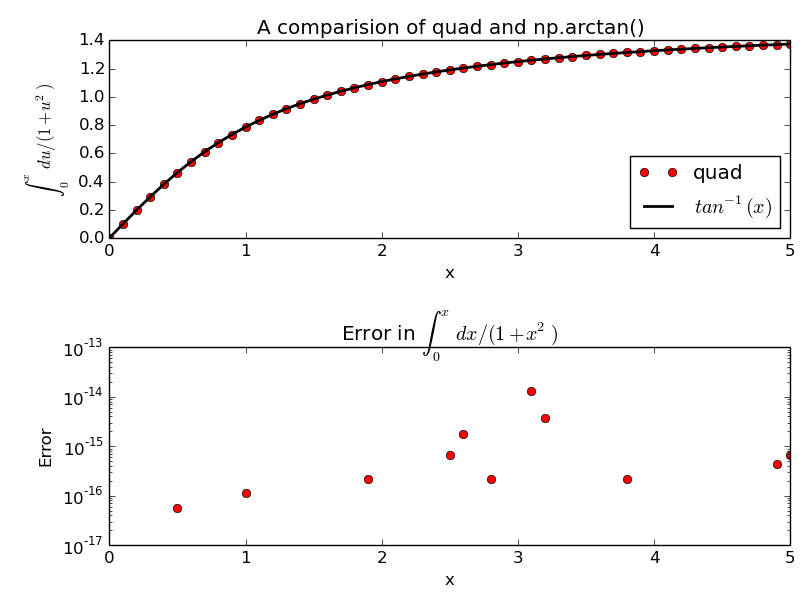
\includegraphics[width= \linewidth]{figure1.png}
		\label{fig:figure1}
		\caption{A plot of $I(x)$ and error}
		\end{figure} 

		The error returned by the quad function is plotted which looks as follows.
		
		\begin{figure}[H]
		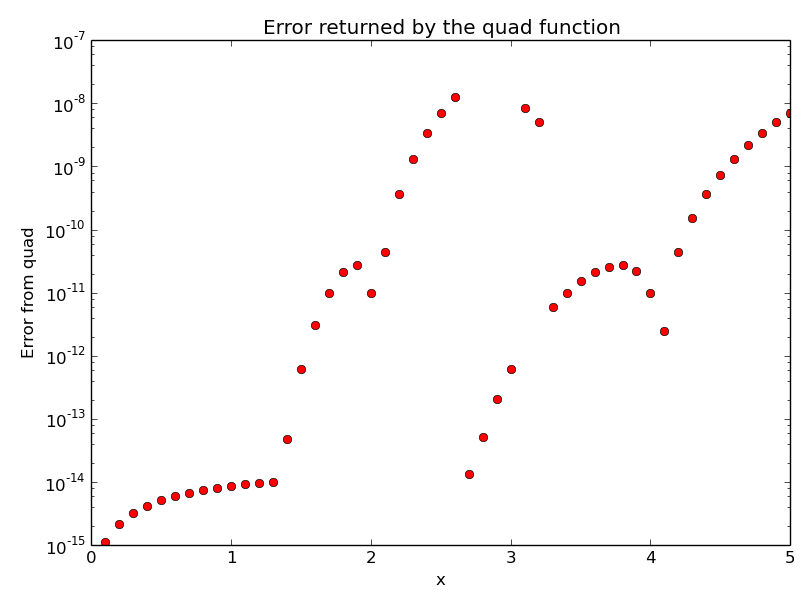
\includegraphics[width=\linewidth]{figure2.png}
		\label{fig:figure2}
		\caption{Error returned by the quad function}
		\end{figure}	

		The table shows values of $tan^{-1}x$ returned by the $quad$ function and the $np.arctan$ function.

			\begin{center}
			
				\begin{longtable}{c|r|r}
				\textbf{Value of $x$} & \textbf{Returned value from quad} &\textbf{Value of $np.arctan$}\\
				\hline

				0.0 & 0.0 & 0.0\\ 
				0.1 & 0.09967 & 0.09967\\ 
				0.2 & 0.1974 & 0.1974\\ 
				0.3 & 0.29146 & 0.29146\\ 
				0.4 & 0.38051 & 0.38051\\ 
				0.5 & 0.46365 & 0.46365\\ 
				0.6 & 0.54042 & 0.54042\\ 
				0.7 & 0.61073 & 0.61073\\ 
				0.8 & 0.67474 & 0.67474\\ 
				0.9 & 0.73282 & 0.73282\\ 
				1.0 & 0.7854 & 0.7854\\ 
				1.1 & 0.83298 & 0.83298\\ 
				1.2 & 0.87606 & 0.87606\\ 
				1.3 & 0.9151 & 0.9151\\ 
				1.4 & 0.95055 & 0.95055\\ 
				1.5 & 0.98279 & 0.98279\\ 
				1.6 & 1.0122 & 1.0122\\ 
				1.7 & 1.03907 & 1.03907\\ 
				1.8 & 1.0637 & 1.0637\\ 
				1.9 & 1.08632 & 1.08632\\ 
				2.0 & 1.10715 & 1.10715\\ 
				2.1 & 1.12638 & 1.12638\\ 
				2.2 & 1.14417 & 1.14417\\ 
				2.3 & 1.16067 & 1.16067\\ 
				2.4 & 1.17601 & 1.17601\\ 
				2.5 & 1.19029 & 1.19029\\ 
				2.6 & 1.20362 & 1.20362\\ 
				2.7 & 1.21609 & 1.21609\\ 
				2.8 & 1.22777 & 1.22777\\ 
				2.9 & 1.23874 & 1.23874\\ 
				3.0 & 1.24905 & 1.24905\\ 
				3.1 & 1.25875 & 1.25875\\ 
				3.2 & 1.26791 & 1.26791\\ 
				3.3 & 1.27656 & 1.27656\\ 
				3.4 & 1.28474 & 1.28474\\ 
				3.5 & 1.2925 & 1.2925\\ 
				3.6 & 1.29985 & 1.29985\\ 
				3.7 & 1.30683 & 1.30683\\ 
				3.8 & 1.31347 & 1.31347\\ 
				3.9 & 1.31979 & 1.31979\\ 
				4.0 & 1.32582 & 1.32582\\ 
				4.1 & 1.33156 & 1.33156\\ 
				4.2 & 1.33705 & 1.33705\\ 
				4.3 & 1.3423 & 1.3423\\ 
				4.4 & 1.34732 & 1.34732\\ 
				4.5 & 1.35213 & 1.35213\\ 
				4.6 & 1.35674 & 1.35674\\ 
				4.7 & 1.36116 & 1.36116\\ 
				4.8 & 1.3654 & 1.3654\\ 
				4.9 & 1.36948 & 1.36948\\ 
				5.0 & 1.3734 & 1.3734\\ 

				\hline
				\addlinespace
				\caption{Values of $tan^{-1}x$}
				\label{tab:table1}

				\end{longtable}
			\end{center}
			
		\item The trapezoid rule is used to achieve results similar to the quad functions. The following code implements this algorithm:
			
			$$I= \left\{
					\begin{array}{ll}
						0 & \quad x = a \\
						0.5(f(a) + f(x_i)) + \sum_{j=2}^{i-1}f(x_j) & \quad x = a+ih
					\end{array}
				\right.
				$$	

		where $f(x)$ is the function to be integrated, $a$ the lower limit, $b$ the upper limit and $h$ the step size. Alternately, we can write out the above algorithm as follows,

		\begin{equation*}
		I_i = h \left(\sum_{j=1}^{i}f(x_j)- \frac{1}{2}(f(x_1) + f(x_i))\right)
		\end{equation*}
			 

		\begin{lstlisting}

		def trapezoid_integrate(a,b,h,f):
			# making the assumption that b-a/h is integral
			avbl_points= np.linspace(a,b,((b-a)/h)+1)	
			values= f(avbl_points)
			integral= []
			integral= h*(np.cumsum(values)- 0.5*( [values[0]]*len(values) + values ))
			return np.array(integral)


		def trapezoid_integrate_for_loop(a,b,h,f):
			# making the assumption that b-a/h is integral		
			avbl_points= np.linspace(a,b,((b-a)/h)+1)						
			values= f(avbl_points)
			integral= []
			for i in range(0,len(values)):
				integral.append(h*(np.sum(values[:i+1])- 0.5*(values[0]+values[len(values[:i+1])-1])))
			return np.array(integral)

		\end{lstlisting}

		The first of these functions vectorises the code whereas the second function iterates through the values separated by h using a for loop. These functions are called in order and print the same output.


		\begin{lstlisting}

		###########
		# Step 5

		import time as t

		# vectorised code
		t1= t.time()
		print trapezoid_integrate(0,5,0.1,function1)
		t2= t.time()
		print t2-t1
		# code with the for trapezoid_integrate_for_loop
		t1= t.time()
		print trapezoid_integrate_for_loop(0,5,0.1,function1)
		t2= t.time()
		print t2-t1

		# vectorised code
		t1= t.time()
		print trapezoid_integrate(0,5,0.0001,function1)
		t2= t.time()
		print t2-t1
		# code with the for trapezoid_integrate_for_loop
		t1= t.time()
		print trapezoid_integrate_for_loop(0,5,0.0001,function1)
		t2= t.time()
		print t2-t1

		\end{lstlisting}

		This is a comparision of the performance of the vectorised code against the for loop and produces the following output.

		\begin{figure}[H]
		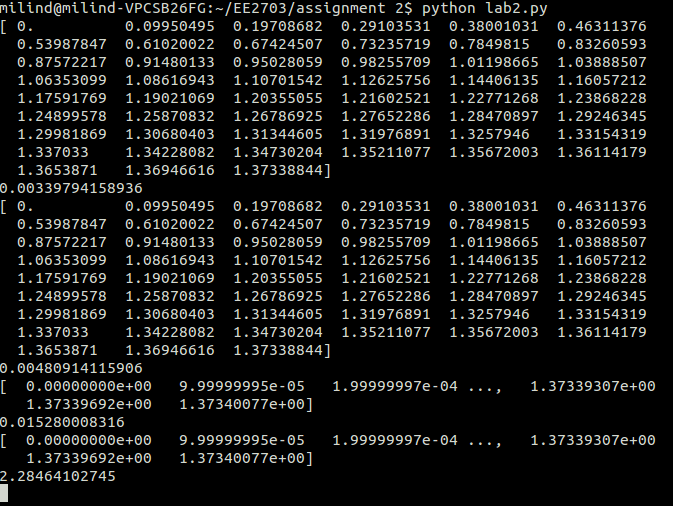
\includegraphics[width= \linewidth]{vector.png}
		\label{fig:vector}
		\caption{Vectorised code vs for-loop as the input size goes up}
		\end{figure}

		Finally, the function $1/(1+x^2)$ is integrated over the range $(0,1)$ several times halving the value of $h$ successively and determining the value of $h$ at which the tolerance value drops below $10^{-8}$. The tolerance is defined as the maximum of the absolute value of the difference between the common points over consecutive values of $h$. This error and the deviation of the function from np.arctan are also plotted as shown in Figure \ref{fig:figure3}.


		\begin{lstlisting}

		#to determine h
		interval_start= 0
		interval_end= 1
		h= 0.1
		hlist=[]

		tolerance= 1
		integrals=[]
		i=1
		error=[]

		integrals.append(trapezoid_integrate( interval_start, interval_end, h, function1))

		while tolerance > 10**(-8):
			h= h/2
			hlist.append(h)
			integrals.append(trapezoid_integrate( interval_start, interval_end, h, function1))
			feed= np.linspace(interval_start, interval_end,((interval_end- interval_start)/h)+1)
			actual_error= max(abs(integrals[i]- np.arctan(feed)))
			error.append( [max( abs( integrals[i][::2]- integrals[i-1])), actual_error])
			i+=1
			tolerance= error[len(error)-1][0]

		error= np.array(error)
		plt.loglog(hlist, error[:,0],"ro",label="estimated error")
		plt.loglog(hlist, error[:,1],"b+",label="actual error")
		plt.legend(loc="lower right")
		plt.show()
		plt.close()
		\end{lstlisting}

		\begin{figure}[H]
		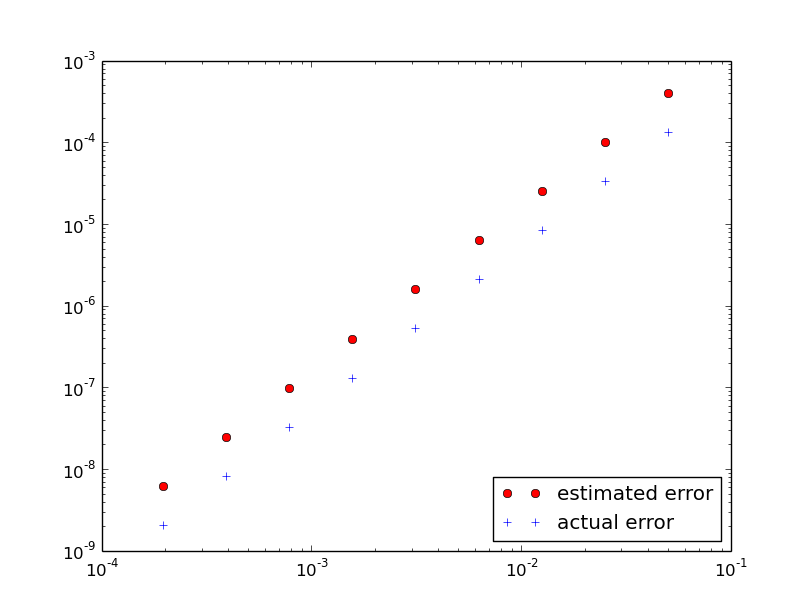
\includegraphics[width= \linewidth]{figure3.png}
		\label{fig:figure3}
		\caption{Estimated error and Exact error} 	
		\end{figure}

	\end{enumerate}

	\section{Conclusion}

	\paragraph{} The $quad$ function and the np.arctan function have marginal difference and this can be seen from Figure 2. The matplotlib library further proves to be invaluable in plotting and visualization of data. We also notice that vectorization of code significantly speeds up code as computation becomes more and more intensive. This can be seen from Figure 4 When the size of $h$ is sufficiently large at 0.1, the code with loops performs nearly as well as the vectorized code, however this is not the case with a much smaller $h$. The trapezoidal rule further serves as a good method to integrate $f(x)$ as Figure \ref{fig:figure3} indicates. Error declines quite significantly with decrease in $h$.

	\paragraph{} In conclusion, methods necessary for scientific computing using python, essentially the scipy and numpy libraries have been outlined with emphasis on the significant advantage of vector methods.


\end{document}